\documentclass{article}
\usepackage{pgfplots}
\usepgfplotslibrary{smithchart}

\begin{document}

This is from http://tex.stackexchange.com/questions/211529/add-circle-to-smith-chart-using-pgf

    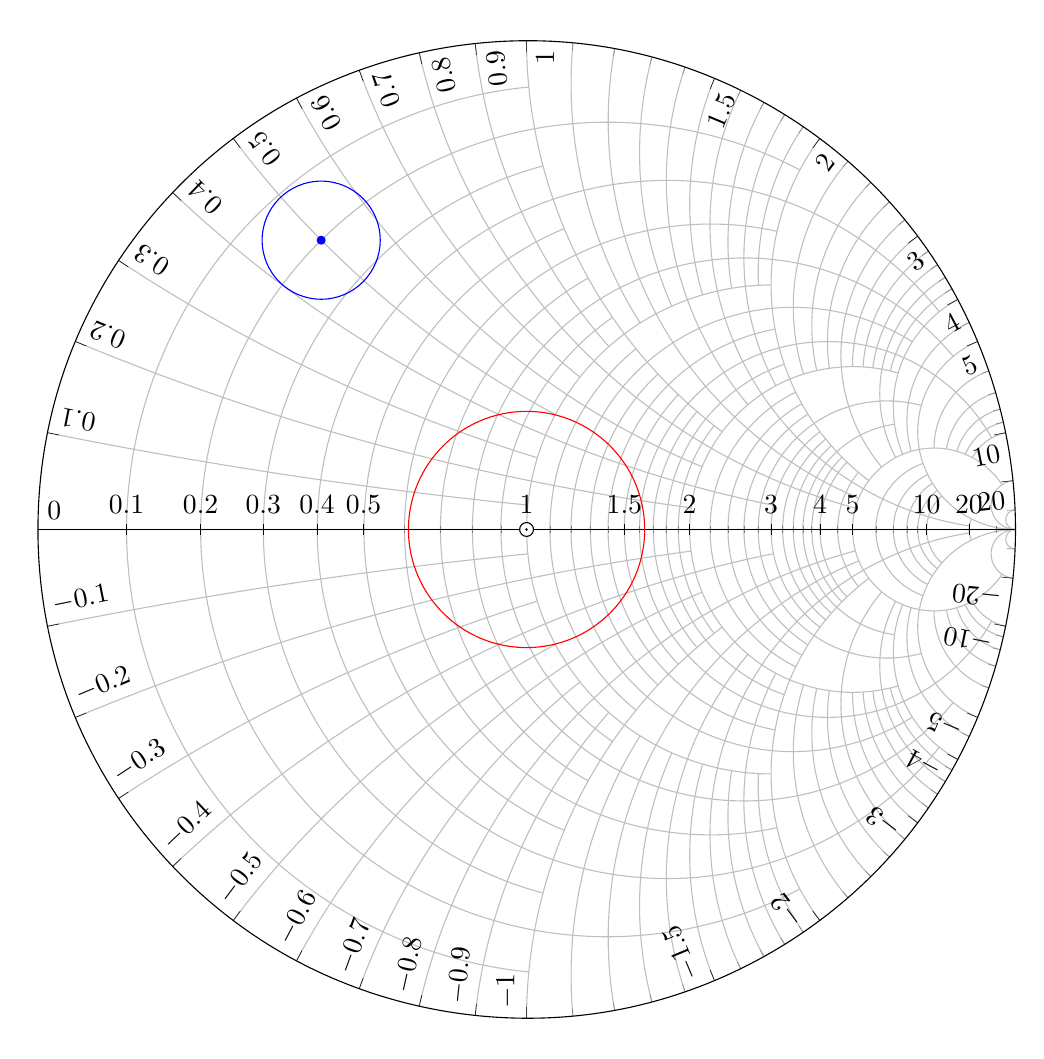
\begin{tikzpicture}
        \begin{smithchart}[width=14cm]
            \path[draw=red] (0pt,0pt) circle (1.5cm);
            \path[draw=blue] (0.2,0.5) circle (0.75cm);
            \path[draw=blue,fill=blue] (0.2,0.5) circle (0.05cm);
        \end{smithchart}
    \end{tikzpicture}

    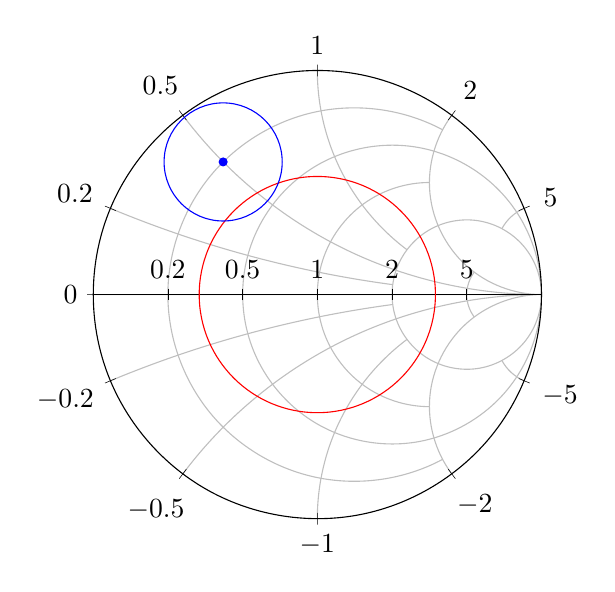
\begin{tikzpicture}
        \begin{smithchart}
            \path[draw=red] (0pt,0pt) circle (1.5cm);
            \path[draw=blue] (0.2,0.5) circle (0.75cm);
            \path[draw=blue,fill=blue] (0.2,0.5) circle (0.05cm);
        \end{smithchart}
    \end{tikzpicture}

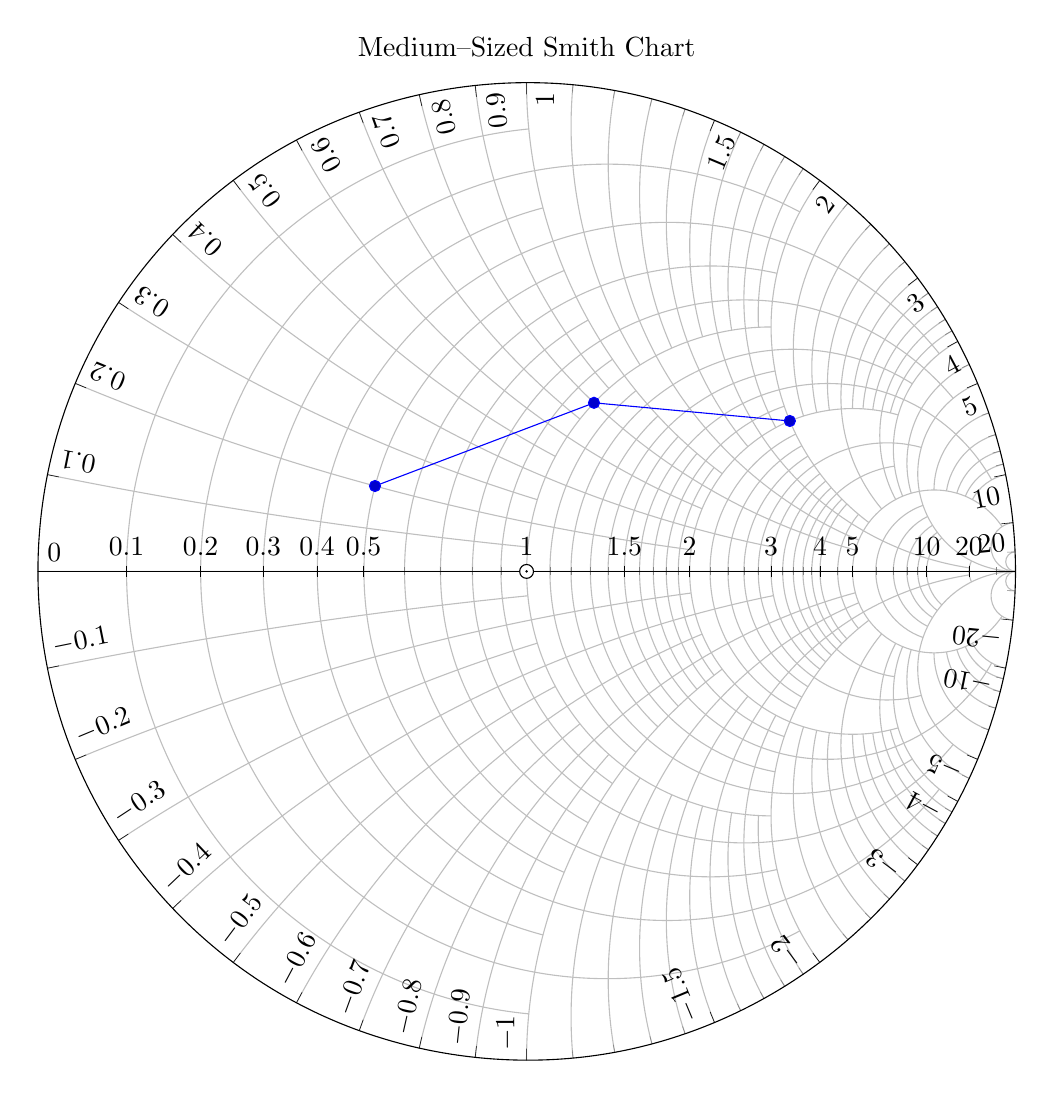
\begin{tikzpicture}
\begin{smithchart}[
title=Medium--Sized Smith Chart,
width=14cm]
\addplot coordinates {(0.5,0.2) (1,0.8) (2,2)};
\end{smithchart}
\end{tikzpicture}

\end{document}
